% SPQR runtime monitor: Rust traces checked against the Lean BraidModel.
% Build: latexmk -lualatex slides.tex
% Figures: scripts/monitor-figures.sh draws fig/*.pdf; docs/monitor.md, section 8.
% Preamble of the SPQR runtime monitor deck, copied from the SpqrBridge decks (spqr-sm-poc/bridge/slides/common).
% Build: latexmk -lualatex slides.tex
\documentclass[aspectratio=169,11pt]{beamer}

\usepackage{fontspec}
\setsansfont{DejaVu Sans}
\directlua{
  luaotfload.add_fallback("leanfallback", {"NotoSansMath:mode=harf;", "STIX Two Math:mode=harf;"})
}
\setmonofont{DejaVu Sans Mono}[Scale=0.9, RawFeature={fallback=leanfallback}]

\usepackage{tikz}
\usepackage{array}
\usetikzlibrary{arrows.meta, positioning, calc, fit, backgrounds, shapes.misc, decorations.pathreplacing}

% Colors. Spec side, impl side, proof, trusted, gap.
\definecolor{refc}{HTML}{2B6CB0}
\definecolor{realc}{HTML}{C05621}
\definecolor{proofc}{HTML}{2F855A}
\definecolor{trustc}{HTML}{718096}
\definecolor{gapc}{HTML}{C53030}
\definecolor{ink}{HTML}{1A202C}
\definecolor{paper}{HTML}{FFFFFF}

\setbeamercolor{normal text}{fg=ink, bg=paper}
\setbeamercolor{frametitle}{fg=ink}
\setbeamercolor{title}{fg=ink}
\setbeamercolor{subtitle}{fg=trustc}
\setbeamercolor{structure}{fg=refc}
\setbeamerfont{frametitle}{size=\Large, series=\bfseries}
\setbeamerfont{subtitle}{size=\footnotesize}
\setbeamertemplate{navigation symbols}{}
\setbeamertemplate{footline}{%
  \hfill\textcolor{trustc}{\scriptsize\insertframenumber/\inserttotalframenumber}\hspace{1.2em}\vspace{0.8em}}

\tikzset{
  >={Stealth[length=2.4mm]},
  box/.style={draw, rounded corners=3pt, thick, align=center, inner sep=5pt, font=\small},
  spec/.style={box, draw=refc, fill=refc!8},
  impl/.style={box, draw=realc, fill=realc!8},
  proof/.style={box, draw=proofc, fill=proofc!10},
  trust/.style={box, draw=trustc, fill=trustc!10},
  gap/.style={box, draw=gapc, fill=gapc!6, dashed},
  tool/.style={box, draw=ink!60, fill=ink!4},
  doc/.style={box, draw=ink!60, fill=paper, double, double distance=1pt},
  flow/.style={->, thick, ink!70},
  proved/.style={<->, very thick, proofc},
  rel/.style={-, very thick, proofc, dashed},
  label/.style={font=\scriptsize, align=center},
}

\newcommand{\code}[1]{\texttt{#1}}
\newcommand{\specside}[1]{\textcolor{refc}{#1}}
\newcommand{\implside}[1]{\textcolor{realc}{#1}}

\author{SPQR runtime monitor}
\date{November 2026}


\title{A runtime monitor for SPQR}
\subtitle{Rust traces checked against the Lean \code{BraidModel}, in the style of SpecMon}


\begin{document}

\begin{frame}
  \titlepage
  \centering
  {\footnotesize\textcolor{trustc}{Inspiration: SpecMon, as used in \emph{From Specs to Apps:
  Verifying and Monitoring Models of Signal and WhatsApp}, ePrint 2026/1979, \S2.2--\S3.}}
\end{frame}

% ---------------------------------------------------------------------------------------------
\begin{frame}[t]{Why a monitor, when we have \code{run\_refines}?}
  \footnotesize
  \begin{itemize}\footnotesize
    \item \code{run\_refines}: for primitives with \code{CodeAgrees P}, every finite run of
      successful calls of the \emph{extracted} Lean code from a related state is a
      \code{BraidModel} run with the same keys and a related end state.
    \item The monitor checks the compiled test build (feature \code{monitor}) on the paths
      that the tests execute. It needs no new extraction.
    \item So it sees what the proof cannot see:
      \begin{itemize}\footnotesize
        \item \textbf{opaque and external functions}: ML-KEM is a hand-written FIPS 203 model,
          HMAC and HKDF are opaque. The monitor uses what the real code returned, and the keys,
          labels and bytes the code passed in;
        \item code patched or left out for extraction: 26 patches, and the SIMD field
          multiplication that runs on CPUs with \code{pclmulqdq};
        \item a primitive call that the model needs and that the code left out, and code that
          changed after the last extraction.
      \end{itemize}
  \end{itemize}
  \centering
  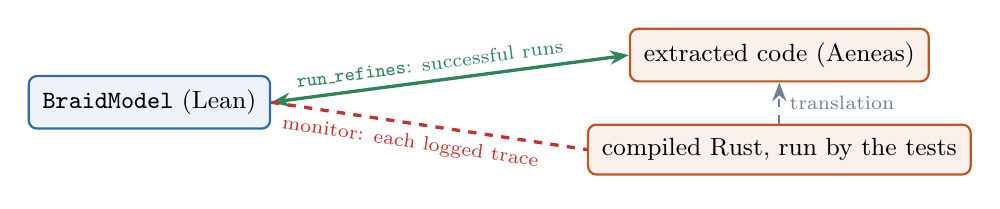
\begin{tikzpicture}[every node/.append style={font=\scriptsize}]
    \node[spec, minimum width=3.0cm] (model) at (0, 0) {\code{BraidModel} (Lean)};
    \node[impl, minimum width=3.4cm] (ext) at (8, 0.6) {extracted code (Aeneas)};
    \node[impl, minimum width=3.4cm] (bin) at (8, -0.6) {compiled Rust, run by the tests};
    \draw[proved] (model.east) -- node[pos=0.45, above, sloped, label, text=proofc] {\code{run\_refines}: successful runs}
      (ext.west);
    \draw[very thick, gapc, dashed] (model.east) -- node[pos=0.45, below, sloped, label, text=gapc]
      {monitor: each logged trace} (bin.west);
    \draw[flow, trustc, dashed] (bin.north) -- node[right, label, text=trustc]
      {translation} (ext.south);
  \end{tikzpicture}
\end{frame}

% ---------------------------------------------------------------------------------------------
\begin{frame}[t]{The pipeline}
  \footnotesize
  \centering
  \vspace{0.8em}
  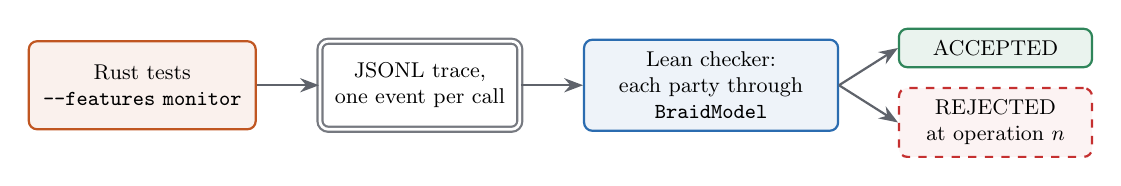
\begin{tikzpicture}[scale=0.86, transform shape, every node/.append style={font=\scriptsize}]
    \node[impl, text width=3.0cm, minimum height=1.3cm] (rust) at (0, 0)
      {Rust tests\\\code{--features monitor}};
    \node[doc, text width=2.6cm, minimum height=1.3cm] (jsonl) at (4.1, 0)
      {JSONL trace,\\one event per call};
    \node[spec, text width=3.4cm, minimum height=1.3cm] (lean) at (8.4, 0)
      {Lean checker:\\each party through \code{BraidModel}};
    \node[proof, text width=2.5cm] (ok) at (12.6, 0.55) {ACCEPTED};
    \node[gap, text width=2.5cm] (rej) at (12.6, -0.55) {REJECTED at operation $n$};
    \draw[flow] (rust) -- (jsonl);
    \draw[flow] (jsonl) -- (lean);
    \draw[flow] (lean.east) -- (ok.west);
    \draw[flow] (lean.east) -- (rej.west);
  \end{tikzpicture}
  \vspace{0.8em}

  \raggedright
  \begin{itemize}\footnotesize
    \item Hooks in \code{src/}, behind the cargo feature \code{monitor}: HMAC, HKDF, ML-KEM,
      decoder results, and each \code{States::send} / \code{recv}.
    \item The Lean checker comes with a theorem: for every $P$ that extends the tables of an
      accepted party, each logged step is the model's step, and the model has a run that emits
      the logged keys.
      Three checks across the parties are not proved: delivery, key agreement, randomness reuse.
    \item With the feature off, the expanded Rust is identical to \code{main}, and all 26
      translation patches still apply. The extraction does not see the hooks.
    \item Event shape, as in SpecMon: $\langle f(\mathit{args}), \mathit{ret}\rangle$.
  \end{itemize}
\end{frame}

% ---------------------------------------------------------------------------------------------
\begin{frame}[t,fragile]{What one operation looks like in the trace}
  \footnotesize
  \vspace{0.4em}
  \begin{itemize}\footnotesize
    \item Each event has a session \code{s}, a party \code{p} and an operation number \code{op}.
      Every operation other than initialization (operation 0) ends with exactly one step event.
  \end{itemize}
  \vspace{0.3em}
{\fontsize{6.5}{7.5}\selectfont
\begin{verbatim}
{"s":1,"p":"A","op":0,"f":"init","args":["a","31"],"ret":null}
{"s":1,"p":"A","op":0,"f":"hkdf","args":["0000..00","0000..31","5369..0001",64],"ret":"5a2bc7b1..."}
{"s":1,"p":"A","op":8,"f":"mlkem.generate","args":["a6413302..."],"ret":["e0234dab...", ...]}
{"s":1,"p":"A","op":8,"f":"hmac","args":["<mac key>","<PROTOCOL_INFO || label || be64(1) || hdr>"],"ret":"..."}
{"s":1,"p":"A","op":8,"f":"States::send","args":["KeysUnsampled",1],
   "ret":{"state":"KeysSampled","epoch":1,"msg":{"epoch":1,"kind":"hdr","index":0,"data":"..."},"key":null}}
{"s":1,"p":"B","op":14,"f":"States::recv","args":["NoHeaderReceived",1,{"epoch":1,"kind":"hdr",...}],
   "ret":{"state":"NoHeaderReceived","epoch":1,"key":null}}
\end{verbatim}
}
  \vspace{0.3em}
  \begin{itemize}\footnotesize
    \item The primitive calls of operation $i$ form a partial table $Q_i$: HMAC, HKDF, KeyGen,
      Encaps1, Encaps2, Decaps, \code{ek\_matches\_header}, decoder results, parity chunks.
    \item The step event gives the observation: the message, the key, the new state name and
      epoch. The logged state name and epoch before the call must match the model's.
  \end{itemize}
\end{frame}

% ---------------------------------------------------------------------------------------------
\begin{frame}[t]{The braid that the checker replays}
  \footnotesize
  \centering
  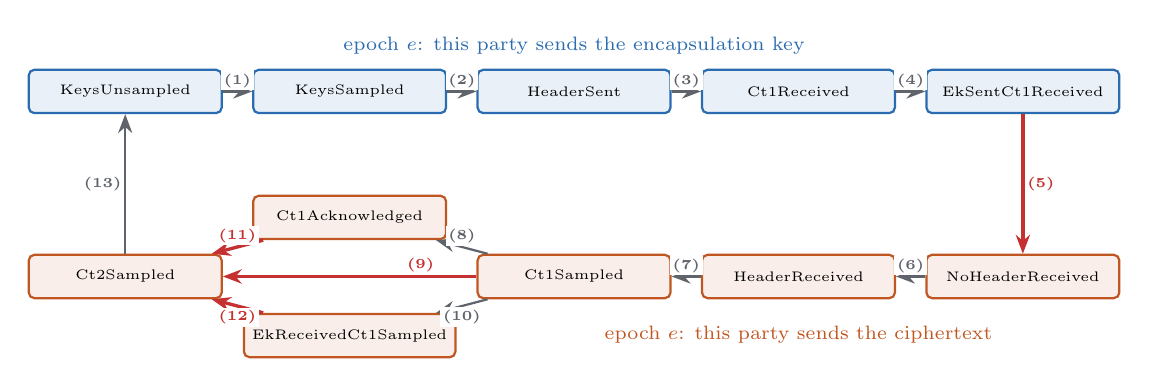
\begin{tikzpicture}[every node/.append style={font=\tiny},
      st/.style={draw, rounded corners=2pt, thick, inner sep=3pt, minimum width=2.45cm,
        minimum height=0.55cm, font=\tiny},
      ek/.style={st, draw=refc, fill=refc!10}, ct/.style={st, draw=realc, fill=realc!10},
      tr/.style={->, thick, ink!70}, mac/.style={->, very thick, gapc},
      n/.style={font=\tiny\bfseries, fill=paper, inner sep=1pt}]
    \node[ek] (KU) at (0, 0) {KeysUnsampled};
    \node[ek] (KS) at (2.85, 0) {KeysSampled};
    \node[ek] (HS) at (5.7, 0) {HeaderSent};
    \node[ek] (C1R) at (8.55, 0) {Ct1Received};
    \node[ek] (ESC) at (11.4, 0) {EkSentCt1Received};
    \node[ct] (NHR) at (11.4, -2.35) {NoHeaderReceived};
    \node[ct] (HR) at (8.55, -2.35) {HeaderReceived};
    \node[ct] (C1S) at (5.7, -2.35) {Ct1Sampled};
    \node[ct] (C1A) at (2.85, -1.6) {Ct1Acknowledged};
    \node[ct] (ERC) at (2.85, -3.1) {EkReceivedCt1Sampled};
    \node[ct] (C2S) at (0, -2.35) {Ct2Sampled};
    \draw[tr] (KU) -- node[above, n] {(1)} (KS);
    \draw[tr] (KS) -- node[above, n] {(2)} (HS);
    \draw[tr] (HS) -- node[above, n] {(3)} (C1R);
    \draw[tr] (C1R) -- node[above, n] {(4)} (ESC);
    \draw[mac] (ESC) -- node[right, n, text=gapc] {(5)} (NHR);
    \draw[tr] (NHR) -- node[above, n] {(6)} (HR);
    \draw[tr] (HR) -- node[above, n] {(7)} (C1S);
    \draw[tr] (C1S) -- node[above, n] {(8)} (C1A);
    \draw[tr] (C1S) -- node[below, n] {(10)} (ERC);
    \draw[mac] (C1S) -- node[pos=0.22, above, n, text=gapc] {(9)} (C2S);
    \draw[mac] (C1A) -- node[above, n, text=gapc] {(11)} (C2S);
    \draw[mac] (ERC) -- node[below, n, text=gapc] {(12)} (C2S);
    \draw[tr] (C2S) -- node[left, n] {(13)} (KU);
    \node[font=\scriptsize, text=refc, anchor=south] at (5.7, 0.35) {epoch $e$: this party sends the encapsulation key};
    \node[font=\scriptsize, text=realc, anchor=north] at (8.55, -2.85) {epoch $e$: this party sends the ciphertext};
  \end{tikzpicture}

  \vspace{0.1em}
  \raggedright
  {\scriptsize
  \renewcommand{\arraystretch}{1.05}
  \begin{tabular}{@{}>{\raggedright}p{4.4cm}>{\raggedright}p{4.4cm}>{\raggedright\arraybackslash}p{4.4cm}@{}}
    (1) send: KeyGen, header MAC & (6) header decoded, verify MAC & (10) ek decoded \\
    (2) first \code{ct1} chunk & (7) send: Encaps1, key of $e$ & \textcolor{gapc}{(11) ek decoded: Encaps2, MAC} \\
    (3) \code{ct1} decoded & (8) ack chunk, \code{ek} incomplete & \textcolor{gapc}{(12) ack: Encaps2, MAC} \\
    (4) first \code{ct2} chunk & \textcolor{gapc}{(9) ek decoded from acks: Encaps2, MAC} & (13) message of epoch $e{+}1$ \\
    \textcolor{gapc}{(5) \code{ct2} decoded: Decaps, verify MAC, key, $e{+}1$} & & \\
  \end{tabular}}
\end{frame}

% ---------------------------------------------------------------------------------------------
\begin{frame}[t]{Checking one step}
  \footnotesize
  \centering
  \vspace{0.4em}
  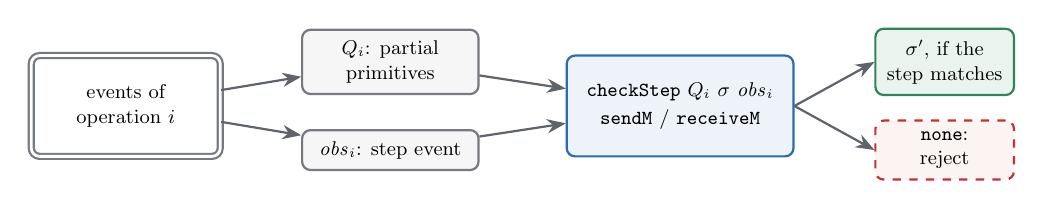
\begin{tikzpicture}[scale=0.8, transform shape, every node/.append style={font=\scriptsize}]
    \node[doc, minimum width=3.0cm, minimum height=1.6cm] (ev) at (0, 0)
      {events of\\operation $i$};
    \node[tool, minimum width=2.8cm] (q) at (4.2, 0.7) {$Q_i$: partial\\primitives};
    \node[tool, minimum width=2.8cm] (obs) at (4.2, -0.7) {$\mathit{obs}_i$: step event};
    \node[spec, minimum width=3.6cm, minimum height=1.6cm] (step) at (8.8, 0)
      {\code{checkStep} $Q_i$ $\sigma$ $\mathit{obs}_i$\\[0.2em]\code{sendM} / \code{receiveM}};
    \node[proof, minimum width=2.2cm] (s2) at (13, 0.7) {$\sigma'$, if the\\step matches};
    \node[gap, minimum width=2.2cm] (none) at (13, -0.7) {\code{none}:\\reject};
    \draw[flow] (ev) -- (q);
    \draw[flow] (ev) -- (obs);
    \draw[flow] (q) -- (step);
    \draw[flow] (obs) -- (step);
    \draw[flow] (step.east) -- (s2.west);
    \draw[flow] (step.east) -- (none.west);
  \end{tikzpicture}
  \vspace{0.6em}

  \raggedright
  \begin{itemize}\footnotesize
    \item \code{OPrims}: the model's primitives with \code{Option} results. A lookup that is not
      in the table is \code{none}, so the step is rejected. There is never a default value.
    \item A primitive lookup of a step uses only the values that the code logged in the same
      \code{States} call; a cached MAC from another call does not count. The step also uses the
      model state from earlier steps, and computes systematic chunks itself.
    \item When it can, the diagnosis names the missing value, for example: ``no hmac call with the key and
      data of the ciphertext MAC (verify\_ct)''.
    \item A receive that the code accepted and the model refuses: ``the model's Receive()
      fails, the code accepted''.
  \end{itemize}
\end{frame}

% ---------------------------------------------------------------------------------------------
\begin{frame}[t,fragile]{What an acceptance means}
  \footnotesize
  \vspace{0.4em}
  \begin{itemize}\footnotesize
    \item \code{Agrees P Q}: $P$ extends the logged values of $Q$, and has the same total fields:
      encoder, decoder, chunk addition, sizes, \code{PROTOCOL\_INFO}, \code{ToBytes}.
  \end{itemize}
{\fontsize{7.5}{8.5}\selectfont
\begin{verbatim}
theorem accepted_alice (h₀ : initAliceM Q₀ ss = some σ₀)
    (h : checkRun σ₀ steps = some σ') (P : Prims Enc Dec Chunk)
    (hA₀ : Agrees P Q₀) (hA : ∀ q ∈ steps, Agrees P q.1) :
    Explains P (initAlice P ss) (steps.map (·.2)) σ' ∧
      Run P (initAlice P ss) σ' (obsKeys (steps.map (·.2)))
\end{verbatim}
}
  \begin{itemize}\footnotesize
    \item For every $P$ that extends the tables built from Alice's log, each logged step is the model's
      step from \code{InitAlice}: a send gives the logged message, key, state name and epoch; a
      receive gives the logged key, state name and epoch, or fails as logged. The model has a
      run that emits the logged keys. Same for Bob.
    \item \code{\#print axioms}: only \code{propext}, \code{Classical.choice} and
      \code{Quot.sound}.
  \end{itemize}
  \vspace{0.3em}
  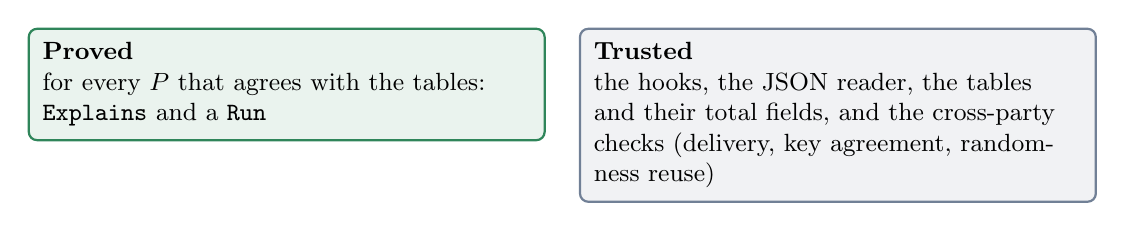
\begin{tikzpicture}[every node/.append style={font=\scriptsize}]
    \node[proof, text width=6.2cm, align=left, anchor=north west] at (0, 0)
      {\textbf{Proved}\\ for every $P$ that agrees with the tables: \code{Explains} and a \code{Run}};
    \node[trust, text width=6.2cm, align=left, anchor=north west] at (7, 0)
      {\textbf{Trusted}\\ the hooks, the JSON reader, the tables and their total fields, and the
      cross-party checks (delivery, key agreement, randomness reuse)};
  \end{tikzpicture}
\end{frame}

% ---------------------------------------------------------------------------------------------
\begin{frame}[t]{An honest run, as the viewer draws it}
  \footnotesize
  \centering
  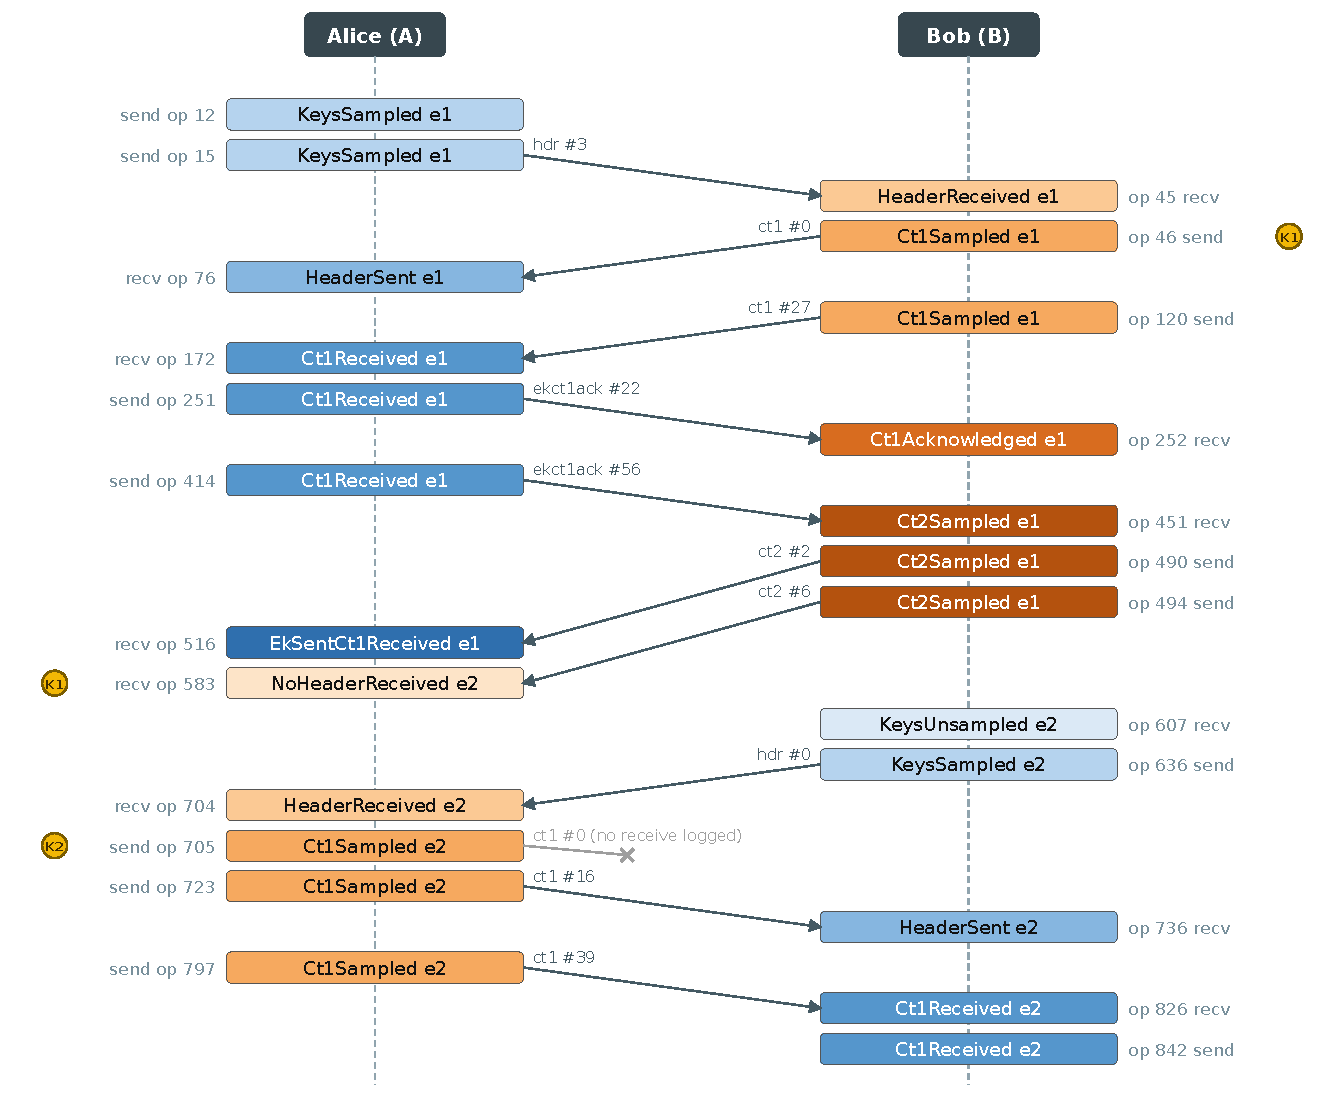
\includegraphics[width=\textwidth,height=6.1cm,keepaspectratio]{fig/honest-seq.pdf}

  \raggedright
  {\scriptsize The start of the \code{chaos} test. Only steps that change state, emit a key, or
  send a message that a kept step receives. \code{(no receive logged)}: no receive of the chunk in the log.
  K1, K2: keys of epochs 1 and 2.}
\end{frame}

% ---------------------------------------------------------------------------------------------
\begin{frame}[t]{The braid over a whole session}
  \footnotesize
  \centering
  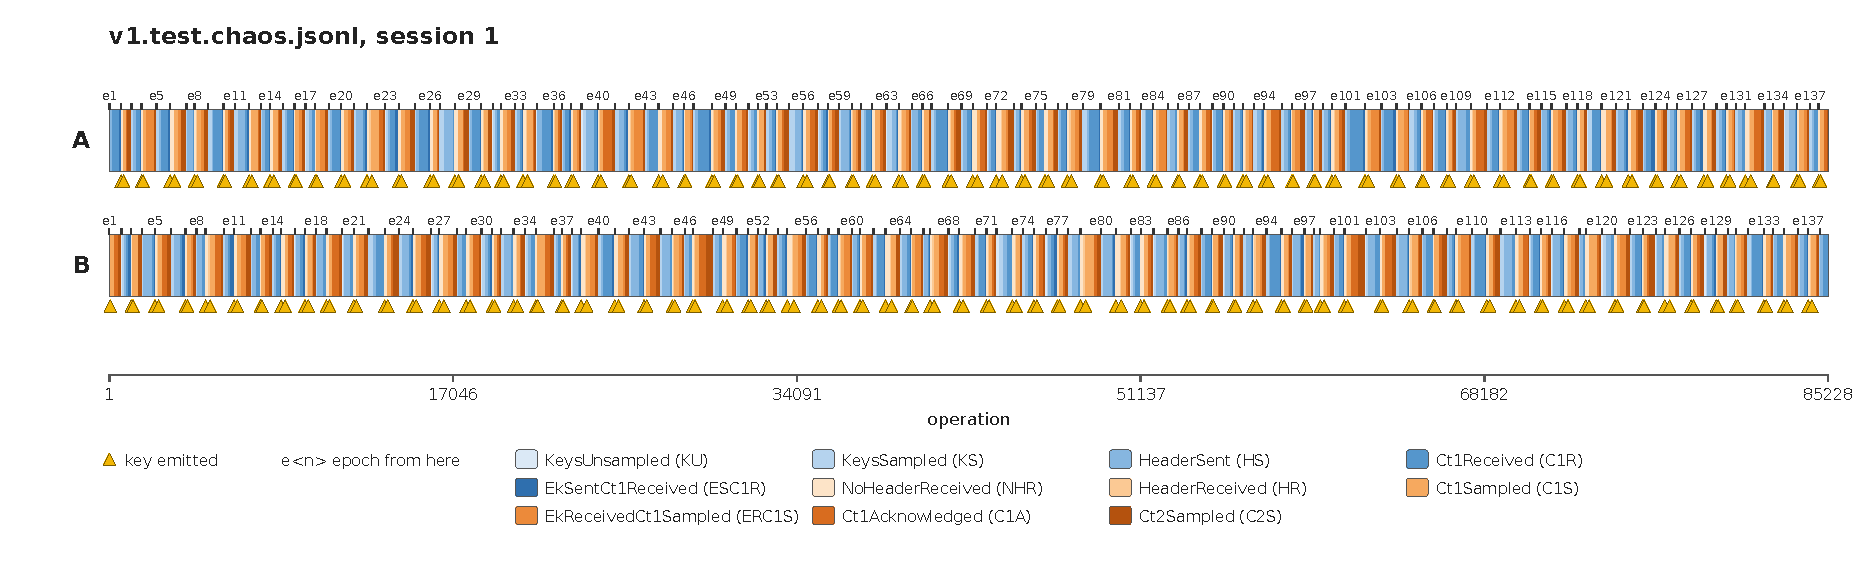
\includegraphics[width=\textwidth]{fig/honest-overview.pdf}

  \raggedright
  \begin{itemize}\footnotesize
    \item Honest code, \code{chaos} test: about 85\,000 operations. All 22 parties of the
      11 test traces are accepted, and key agreement holds in all 11 sessions.
    \item Blue and orange swap in each epoch: that is the braid.
  \end{itemize}
\end{frame}

% ---------------------------------------------------------------------------------------------
\begin{frame}[t]{Mutants: \code{cargo test} passes, the monitor rejects}
  \scriptsize
  \vspace{0.3em}
  \centering
  \renewcommand{\arraystretch}{1.1}
  \begin{tabular}{>{\raggedright}p{0.6cm} >{\raggedright}p{6.0cm} >{\centering}p{1.7cm} >{\raggedright\arraybackslash}p{4.2cm}}
    & \textbf{Change in \code{src/}} & \textbf{\code{cargo test}} & \textbf{Monitor (22 parties)} \\
    \hline
    M1 & \code{verify\_ct} call deleted (scenario 0) & passes & \textcolor{gapc}{22/22 rejected} at (5) \\
    R1 & \code{mac\_ct} keys the HMAC with \code{root\_key} (copy-paste) & passes & \textcolor{gapc}{22/22 rejected} \\
    R2 & \code{mac\_ct} encodes the epoch with \code{to\_le\_bytes} & passes & \textcolor{gapc}{22/22 rejected} \\
    R3 & both sides MAC \code{ct2} only, not \code{ct1}\,$\|$\,\code{ct2} & passes & \textcolor{gapc}{22/22 rejected} \\
    R4 & \code{let \_ = verify\_ct(...)}: result dropped & passes & accepted on honest traces;
      \textcolor{gapc}{rejected} under tampering \\
    M2 & \code{verify\_hdr} skipped & passes & \textcolor{gapc}{rejected} at (6) \\
    M6 & header MAC with the ciphertext label & passes & \textcolor{gapc}{rejected} at (1) / (6) \\
    M5 & KeyGen randomness fixed & passes & model accepts; reuse check \textcolor{gapc}{fails} \\
  \end{tabular}
  \vspace{0.3em}

  \raggedright
  \begin{itemize}\footnotesize
    \item R1--R3 change both parties the same way. The parties still agree on keys, so no test
      notices. The monitor sees that the logged MAC input is not the input the model requires.
  \end{itemize}
\end{frame}

% ---------------------------------------------------------------------------------------------
\begin{frame}[t]{M1: the \code{verify\_ct} call deleted}
  \footnotesize
  \centering
  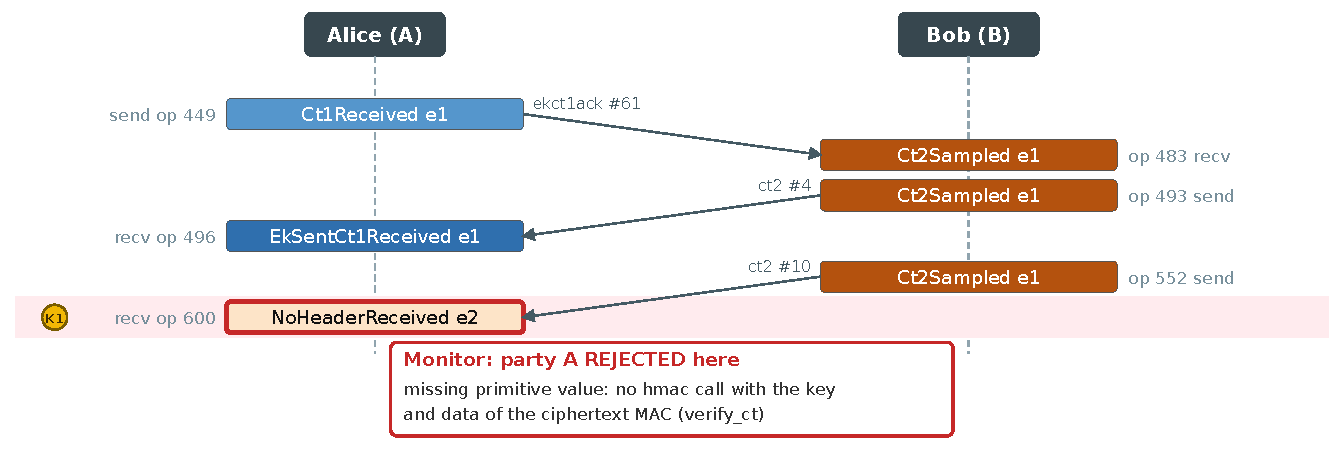
\includegraphics[width=\textwidth,height=6.1cm,keepaspectratio]{fig/m1-seq-a.pdf}

  \raggedright
  {\scriptsize Alice decodes \code{ct2} and moves to epoch 2, but the operation has no HMAC call
  for the ciphertext MAC. Transition (5) needs one.}
\end{frame}

% ---------------------------------------------------------------------------------------------
\begin{frame}[t]{R2: little-endian epoch in the ciphertext MAC}
  \footnotesize
  \centering
  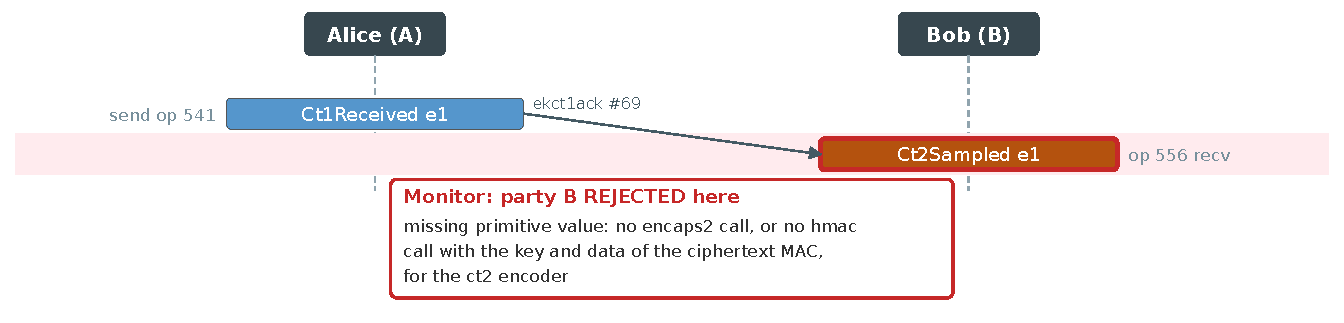
\includegraphics[width=\textwidth,height=5.0cm,keepaspectratio]{fig/r2-seq-b.pdf}

  \raggedright
  \begin{itemize}\footnotesize
    \item Bob is caught first, when he builds the \code{ct2} encoder: the HMAC call has
      other data than $\code{PROTOCOL\_INFO} \| \mathit{label} \| \code{be64}(e) \| \mathit{ct}$.
      Alice is caught later, at (5).
    \item R1 and R3 are also rejected where the HMAC input first differs. The message names a
      missing value, and depends on the transition; it does not say which part of the input
      differs.
  \end{itemize}
\end{frame}

% ---------------------------------------------------------------------------------------------
\begin{frame}[t]{Where the rejections fall in the session}
  \footnotesize
  \centering
  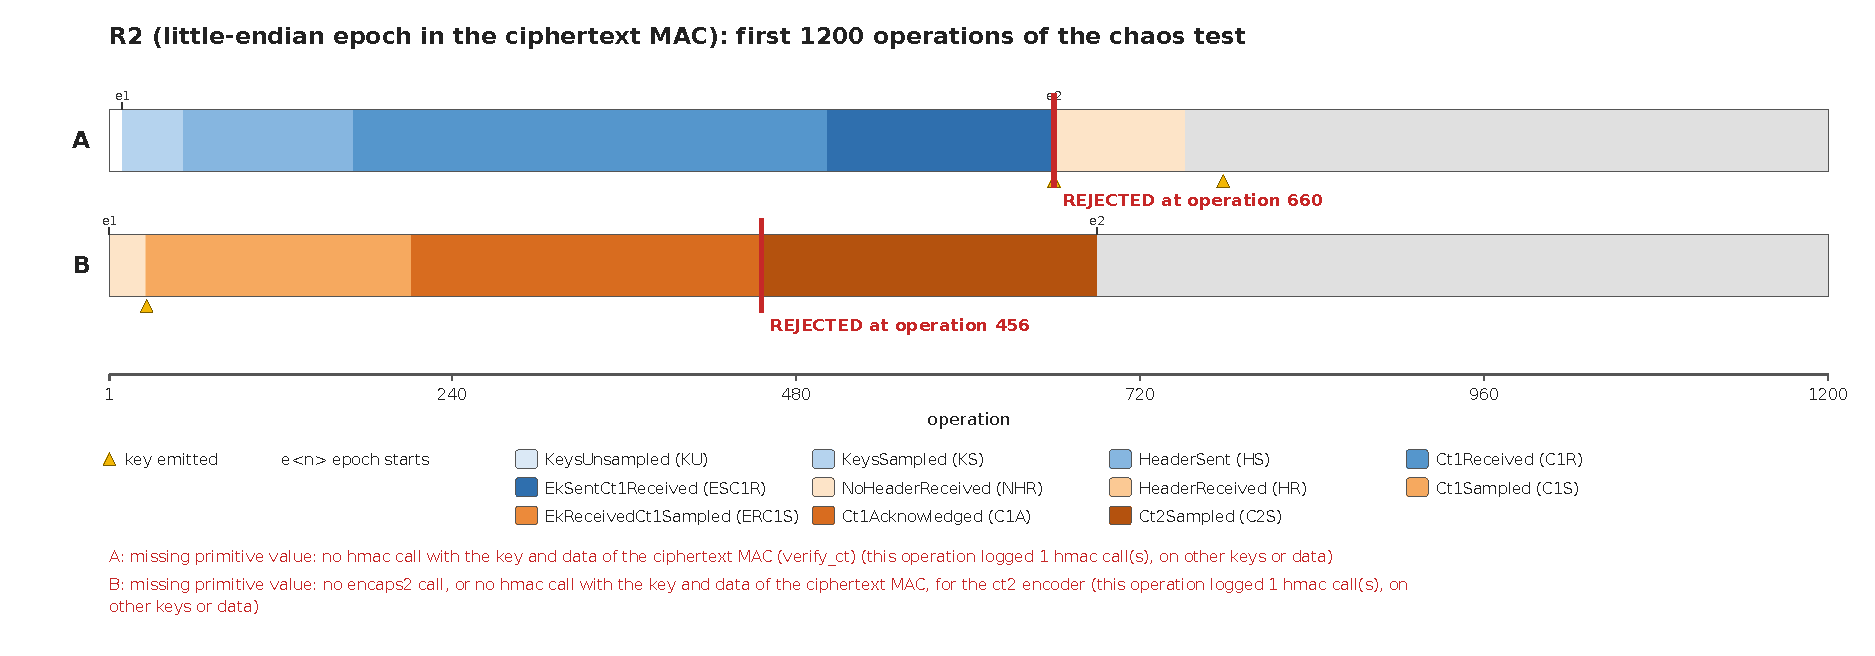
\includegraphics[width=\textwidth]{fig/r2-overview.pdf}

  \raggedright
  {\scriptsize R2, first 1200 operations. After a rejection, the monitor stops checking that
  party (grey). Both parties are caught in epoch 1.}
\end{frame}

% ---------------------------------------------------------------------------------------------
\begin{frame}[t]{R4: a dropped verification result}
  \footnotesize
  \vspace{0.3em}
  \begin{itemize}\footnotesize
    \item \code{let \_ = auth.verify\_ct(...)} instead of \code{...?}. Every MAC in an honest
      run is good, so the monitor accepts R4 on honest traces.
    \item A tampering driver changes one byte of a \code{Hdr} or \code{Ct2} chunk in transit.
  \end{itemize}
  \centering
  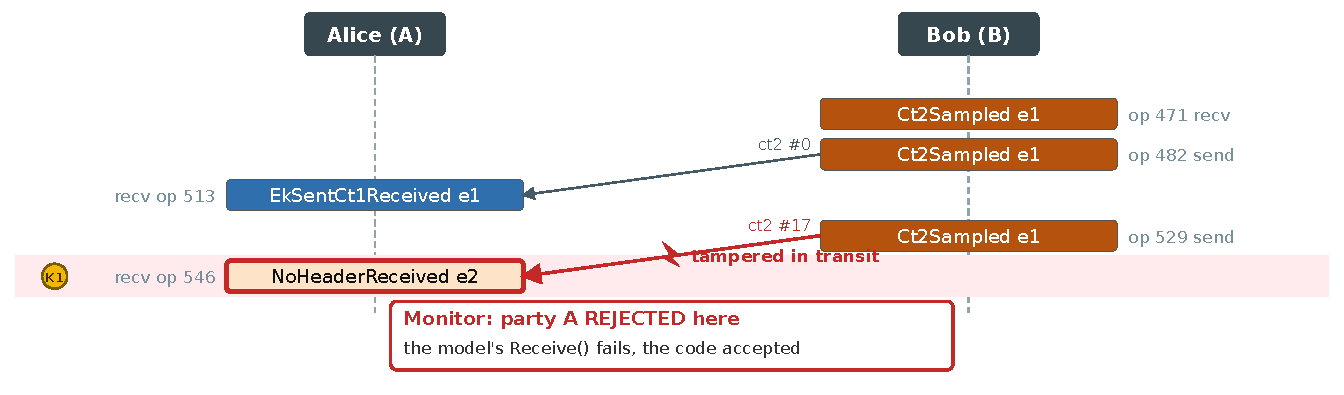
\includegraphics[width=\textwidth,height=4.6cm,keepaspectratio]{fig/r4-seq-a.pdf}

  \raggedright
  {\scriptsize The model's \code{Receive()} fails, the mutant accepts and emits K1. The honest
  code fails at the MAC check and keeps its state: all 36 parties accepted.}
\end{frame}

% ---------------------------------------------------------------------------------------------
\begin{frame}[t]{Checks across the two parties (not proved)}
  \footnotesize
  \vspace{0.6em}
  \begin{itemize}\footnotesize
    \item \textbf{Delivery}: every received message was sent by the peer, as a multiset. A
      tampered copy must match a \code{tamper} event of the same operation: same epoch, kind,
      chunk index and length.
    \item \textbf{Key agreement}: each party logs at most one secret per epoch, and when both
      parties log one for an epoch, they are equal. An epoch with one party's secret only is
      listed as incomplete. It reads the step events, also of a rejected party.
    \item \textbf{Randomness reuse}: no two KeyGen or Encaps1 calls of a session take the same
      randomness.
  \end{itemize}
  \vspace{0.8em}
  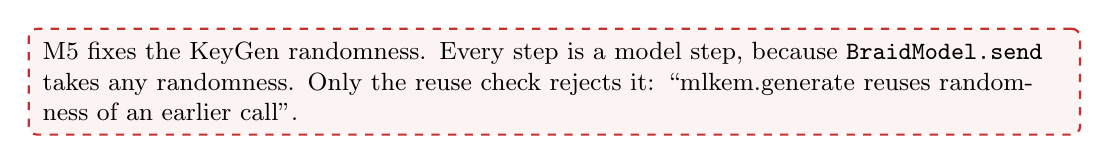
\begin{tikzpicture}[every node/.append style={font=\scriptsize}]
    \node[gap, text width=13cm, align=left] at (0, 0)
      {M5 fixes the KeyGen randomness. Every step is a model step, because
      \code{BraidModel.send} takes any randomness. Only the reuse check rejects it:
      ``mlkem.generate reuses randomness of an earlier call''.};
  \end{tikzpicture}
  \vspace{0.6em}
  \begin{itemize}\footnotesize
    \item Under R4 with tampering, the key agreement check also fails: ``epoch 1: the parties'
      secrets differ''.
  \end{itemize}
\end{frame}

% ---------------------------------------------------------------------------------------------
\begin{frame}[t]{Could a model checker show the traces? UPPAAL}
  \footnotesize
  \begin{columns}[T]
    \begin{column}{0.55\textwidth}
      \centering
      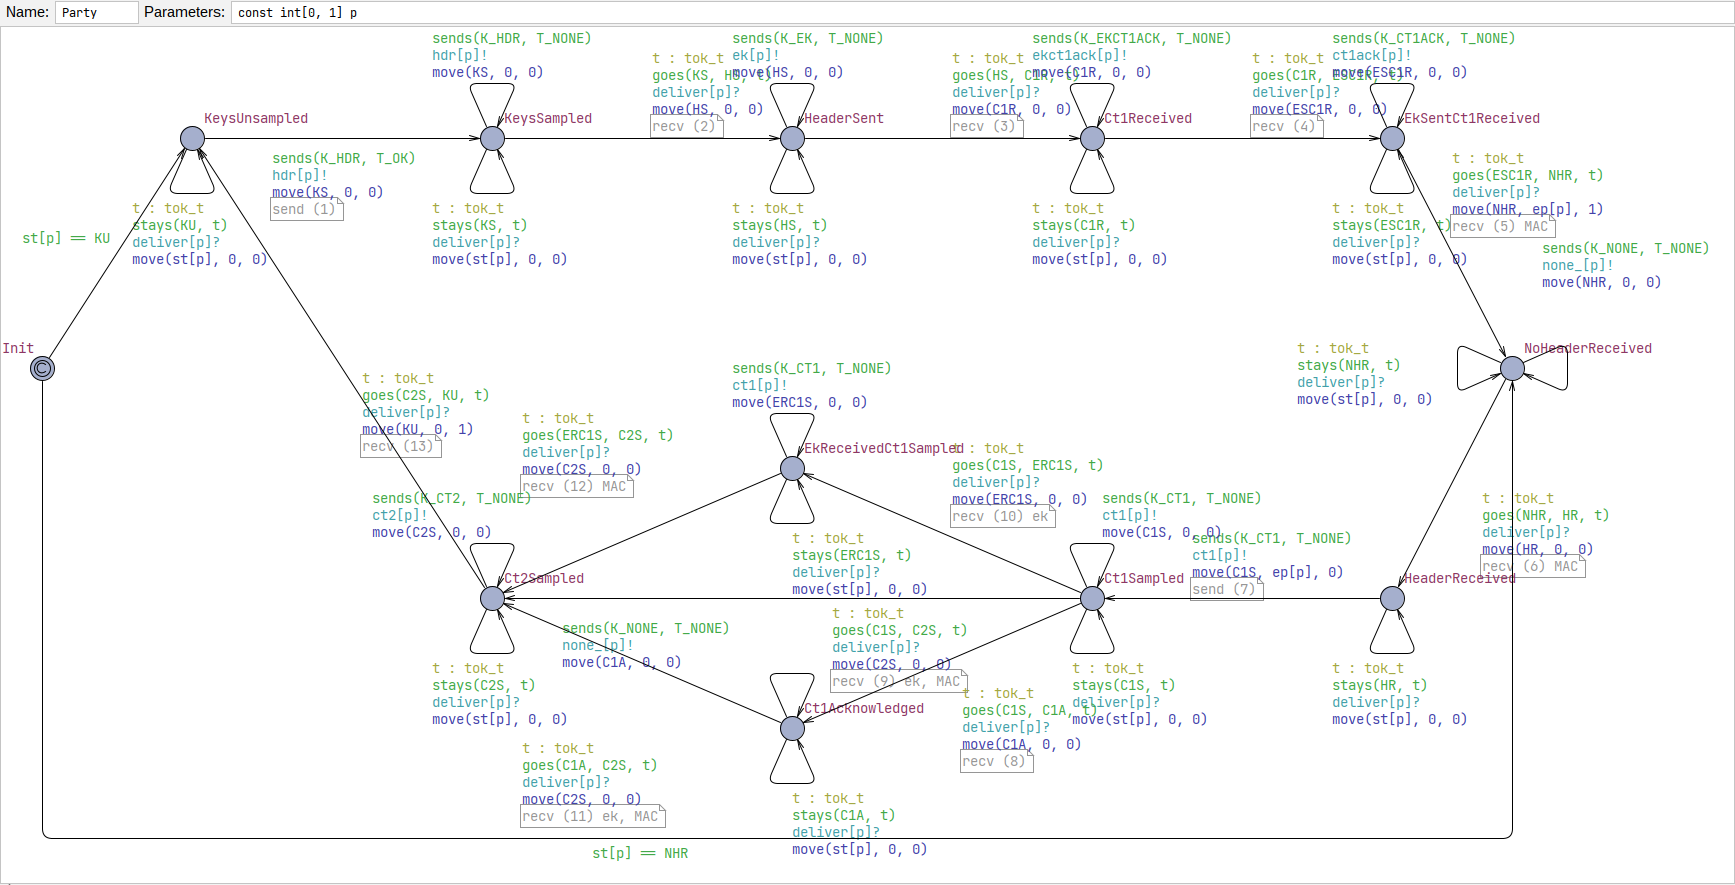
\includegraphics[width=\textwidth]{fig/uppaal-party.png}\\
      {\scriptsize The \code{Party} template: 11 states, transitions (1)--(13).}
    \end{column}
    \begin{column}{0.42\textwidth}
      \begin{itemize}\footnotesize
        \item A script turns a trace into an observer automaton. \code{E<> Obs.done} holds if
          the prefix is a run; otherwise \code{sup: matched} gives the first unmatched step.
        \item In the comparison of the guide, UPPAAL rejects M1, R2, R3 and R4 at the same
          operation as the Lean monitor.
        \item The message sequence chart of a real trace has hundreds of rows and no zoom-out.
        \item No clocks are needed: the braid has no timing.
      \end{itemize}
    \end{column}
  \end{columns}
\end{frame}

% ---------------------------------------------------------------------------------------------
\begin{frame}[t]{Could a model checker show the traces? Veil}
  \footnotesize
  \begin{itemize}\footnotesize
    \item A second braid model, written by hand in Veil's language. No link to
      \code{BraidModel}.
    \item The script checks windows of 12 steps, each from the logged state. For M1, R2 and R3
      the first failing window holds the Lean monitor's rejection. Veil misses R4.
  \end{itemize}
  \vspace{0.8em}
  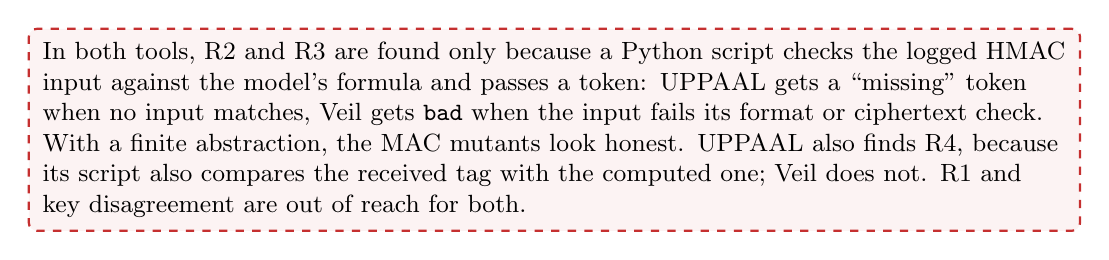
\begin{tikzpicture}[every node/.append style={font=\scriptsize}]
    \node[gap, text width=13cm, align=left] at (0, 0)
      {In both tools, R2 and R3 are found only because a Python script checks the logged HMAC
      input against the model's formula and passes a token: UPPAAL gets a ``missing'' token when
      no input matches, Veil gets \code{bad} when the input fails its format or ciphertext check. With a finite
      abstraction, the MAC mutants look honest. UPPAAL also finds R4, because its script also
      compares the received tag with the computed one; Veil does not. R1 and key disagreement
      are out of reach for both.};
  \end{tikzpicture}
\end{frame}

% ---------------------------------------------------------------------------------------------
\begin{frame}[t]{Three ways to look at the same rejection}
  \footnotesize
  \centering
  \vspace{0.2em}
  \renewcommand{\arraystretch}{1.0}
  \begin{tabular}{>{\raggedright}p{2.6cm} >{\raggedright}p{3.1cm} >{\raggedright}p{3.1cm} >{\raggedright\arraybackslash}p{3.1cm}}
    & \textbf{Lean monitor} & \textbf{UPPAAL} & \textbf{Veil} \\
    \hline
    model & \code{BraidModel} itself & second model & second model \\
    data & messages, keys, primitive values & tokens & tokens \\
    soundness theorem & yes, for every $P$ that extends the tables & no & no \\
    finds M1 & yes & yes & yes \\
    finds R1 & yes & no & no \\
    finds R2, R3 & yes & with a byte check in Python & with a byte check in Python \\
    finds R4 (tampering) & yes & with a byte check in Python & no \\
    checked & the log, up to the first failed step & prefix, one party & prefix, in windows \\
    picture & custom viewer & automaton, MSC & window verdict, rejected operation \\
  \end{tabular}
  \vspace{0.6em}

  \raggedright
  \begin{itemize}\footnotesize
    \item The model checkers add a picture of the automaton. For traces, the custom viewer reads better.
  \end{itemize}
\end{frame}

% ---------------------------------------------------------------------------------------------
\begin{frame}[t]{Limits and next steps}
  \footnotesize
  \vspace{0.2em}
  \begin{itemize}\footnotesize
    \item The monitor checks test executions of the chunked \code{States} machine. It does not
      observe \code{lib.rs} \code{send} / \code{recv}, \code{chain.rs} or the prost state codec.
    \item It takes the primitives' behavior from the log. A wrong HMAC that both parties share
      is accepted, if its inputs are right.
    \item Decoder results and parity chunks are trusted logged values; only the systematic
      chunks are recomputed.
    \item The tampering driver changes only \code{Hdr} and \code{Ct2} chunk bytes.
  \end{itemize}
  \vspace{0.2em}
  \textbf{Next}
  \begin{itemize}\footnotesize
    \item Hooks in \code{lib.rs} would cover the state codec, which \code{run\_refines} does not.
    \item A native build of the checker: the interpreter takes about 4 minutes for all traces.
  \end{itemize}
\end{frame}

\end{document}
